% ======================================================================
%  FYS4480/FYS9480  Quantum mechanics for many-particle systems
%  Week 40, October 1-2, 2026
%  Lecture slides (Beamer).  Thursday: 2 x 45 min,  Friday: 2 x 45 min.
%
%  Sources: chapterDMRG.tex (chapter 11 of the lecture notes).  Thursday:
%  a ten-minute repetition of week 39 (Thouless' theorem and the stability
%  matrix, sections 6.7 and 6.10), then sections 11.1-11.2 (entanglement
%  across a cut, area laws, the MPS from L-1 SVDs, bond dimension,
%  truncation).  Friday: section 11.2 (canonical forms, transfer matrix),
%  11.3-11.4 (matrix product operators, MPS arithmetic) and 11.7
%  (Jordan-Wigner).  Also chapter 1, sections 1.28-1.31 (SVD, Schmidt) and
%  chapter 4 (pairing, Hubbard, Heisenberg).
%  Exercises: suggested set for week 40 (stability matrix by Wick's theorem,
%  positive semidefinite matrices) and answers to
%  the week-39 set, at the end.
%  Companion program: BookPrograms/chapterdmrg/dmrg.py
%
%  Slide discipline: one claim per frame, the equation or table that
%  carries it, and a few short bullets.  The prose lives in chapter 11 of
%  the lecture notes, not here.  Preamble and box macros as in week39.tex.
%
%  Build:  pdflatex week40.tex  (twice)
%  Handout (no overlays):  replace \documentclass[...] by
%           \documentclass[handout,aspectratio=169]{beamer}
% ======================================================================
\documentclass[aspectratio=169,10pt]{beamer}

% ---------------------------------------------------------------- packages
\usepackage[utf8]{inputenc}
\usepackage[T1]{fontenc}
% \usepackage{lmodern}  % optional; uncomment if installed
\usepackage{amsmath,amssymb,bm,mathtools}
\usepackage{booktabs}
\usepackage{tcolorbox}
\usepackage{listings}
\usepackage{hyperref}
\usepackage{tikz}
\usetikzlibrary{positioning,arrows.meta,decorations.markings,shapes.misc}
\usetikzlibrary{tikzmark}

% ---------------------------------------------------------------- look
\usetheme{default}
\useinnertheme{rectangles}
\setbeamertemplate{navigation symbols}{}
\definecolor{uioblue}{RGB}{18,52,86}
\definecolor{teal}{RGB}{0,128,128}
\definecolor{warm}{RGB}{181,73,36}
\definecolor{paleblue}{RGB}{232,240,248}
\definecolor{paleteal}{RGB}{228,244,244}
\definecolor{palewarm}{RGB}{252,238,230}
\setbeamercolor{structure}{fg=uioblue}
\setbeamercolor{title}{fg=uioblue}
\setbeamercolor{frametitle}{fg=uioblue,bg=white}
\setbeamercolor{section in toc}{fg=uioblue}
\setbeamercolor{alerted text}{fg=warm}
\setbeamercolor{block title}{fg=white,bg=uioblue}
\setbeamercolor{block body}{bg=paleblue}
\setbeamercolor{block title example}{fg=white,bg=teal}
\setbeamercolor{block body example}{bg=paleteal}
\setbeamerfont{frametitle}{size=\large,series=\bfseries}
\setbeamerfont{title}{size=\LARGE,series=\bfseries}
\setbeamertemplate{frametitle}{%
  \vspace*{0.6em}\insertframetitle\par
  \vspace*{-0.2em}{\color{teal}\rule{\textwidth}{0.6pt}}}
\setbeamertemplate{footline}{%
  \hbox{\begin{beamercolorbox}[wd=\paperwidth,ht=2.4ex,dp=1.2ex,leftskip=1em,rightskip=1em]{structure}%
  \footnotesize FYS4480/9480 -- Week 40 \hfill \insertsection \hfill \insertframenumber/\inserttotalframenumber
  \end{beamercolorbox}}}
\setbeamertemplate{itemize items}[circle]
\setbeamertemplate{enumerate items}[default]
\setbeamertemplate{section page}{%
  \begin{centering}
    {\usebeamerfont{section title}\usebeamercolor[fg]{title}\LARGE\bfseries\insertsection\par}
    \vspace{0.5em}{\color{teal}\rule{0.5\textwidth}{1pt}}
  \end{centering}}
\AtBeginSection[]{\frame{\sectionpage}}

% ---------------------------------------------------------------- boxes
% (as in week39.tex)
\newcounter{thinkctr}
\newcommand{\thinkq}[2]{%
  \stepcounter{thinkctr}%
  \begin{tcolorbox}[colback=palewarm,colframe=warm,title={\bfseries Pause to think \#\thethinkctr\hfill\mdseries\small(about #1 min -- discuss with your neighbour)},fonttitle=\bfseries]
  #2
  \end{tcolorbox}}
\newcommand{\thinka}[1]{%
  \begin{tcolorbox}[colback=paleteal,colframe=teal,title={\bfseries Answer to pause \#\thethinkctr}]
  #1
  \end{tcolorbox}}
\newcommand{\mbbox}[1]{%
  \begin{tcolorbox}[colback=paleblue,colframe=uioblue,title={\bfseries Many-body connection}]
  #1
  \end{tcolorbox}}
\newcommand{\qcbox}[1]{%
  \begin{tcolorbox}[colback=paleteal,colframe=teal,title={\bfseries Quantum computing connection}]
  #1
  \end{tcolorbox}}
\newcommand{\warnbox}[1]{%
  \begin{tcolorbox}[colback=palewarm,colframe=warm,title={\bfseries A trap to avoid}]
  #1
  \end{tcolorbox}}

% ---------------------------------------------------------------- code
\lstset{language=Python,basicstyle=\ttfamily\scriptsize,
  keywordstyle=\color{uioblue}\bfseries,commentstyle=\color{teal},
  stringstyle=\color{warm},showstringspaces=false,columns=fullflexible,
  frame=single,rulecolor=\color{paleblue},backgroundcolor=\color{white},
  breaklines=true}

% ---------------------------------------------------------------- macros
\newcommand{\ket}[1]{\vert #1\rangle}
\newcommand{\bra}[1]{\langle #1\vert}
\newcommand{\braket}[2]{\langle #1\vert #2\rangle}
\newcommand{\element}[3]{\langle #1\vert #2\vert #3\rangle}
\newcommand{\ketbra}[2]{\vert #1\rangle\langle #2\vert}
\newcommand{\dd}{\mathrm{d}}
\newcommand{\Det}[1]{\vert\bm{#1}\vert}
\DeclareMathOperator{\tr}{tr}
\DeclareMathOperator{\sgn}{sgn}
% normal ordering with respect to the reference determinant |c>
\newcommand{\nc}[1]{\bigl\{#1\bigr\}}
\newcommand{\bigO}{\mathcal{O}}
% tensor-network notation, as in the lecture notes
\newcommand{\bmat}[1]{\bm{#1}}
\newcommand{\Amat}[1]{\bm{A}^{#1}}
\newcommand{\Bmat}[1]{\bm{B}^{#1}}
\newcommand{\hH}{\hat{H}}
\newcommand{\ad}[1]{a_{#1}^{\dagger}}

% ---------------------------------------------------------------- diagrams
\tikzset{
  tens/.style={draw=uioblue,fill=paleblue,thick,rounded corners=1pt,minimum size=7mm,font=\small},
  mpo/.style={draw=warm,fill=palewarm,thick,rounded corners=1pt,minimum size=7mm,font=\small},
  leg/.style={thick,uioblue},
  dlab/.style={font=\scriptsize},
  every picture/.style={scale=0.8,baseline=(current bounding box.center)}
}

\graphicspath{{../BookFigures/}{./}}

% ---------------------------------------------------------------- title
\title{Matrix product states: the Schmidt decomposition at every bond}
\subtitle{FYS4480/FYS9480 -- Week 40, October 1--2, 2026}
\author{Cecilie Glittum}
\institute{Department of Physics,\\
University of Oslo, Norway}
\date{}

\begin{document}

\begin{frame}[plain]
  \vspace*{0.4em}{\setbeamerfont{title}{size=\Large,series=\bfseries}\titlepage}
  \vfill
  \begin{center}\scriptsize
  Thursday October 1: ten minutes of repetition -- Thouless' theorem and the stability matrix; then entanglement across a cut, area laws, and the matrix product state from $L-1$ singular value decompositions\\
  Friday October 2: canonical forms, the transfer matrix and the cost of contractions; matrix product operators as finite-state automata; adding, applying and compressing; fermions on a chain\\[0.2em]
  Reading: these slides; lecture notes chapter 11, sections 11.1--11.4 and 11.7 (chapter 6, sections 6.7 and 6.10 for the repetition); chapter 1, sections 1.28--1.31. Code: \texttt{BookPrograms/chapterdmrg/dmrg.py}\\[0.4em]
  \end{center}
\end{frame}

\begin{frame}[shrink=5]{Plan for week 40}
  \scriptsize
  \begin{block}{Thursday October 1, $2\times45$ min: from entanglement to matrix product states}
    \begin{itemize}
      \item Repetition (10 min): Thouless' theorem, the energy to second order, the stability matrix $\hat M$ and its blocks $\Delta$, $A$, $B$; Lipkin unstable, pairing stable and useless (sections 6.7, 6.10--6.11)
      \item A third strategy: restrict the \emph{entanglement}, not the basis; the methods in one table (chapter 11, introduction)
      \item A bipartite state is a matrix; Schmidt decomposition $=$ SVD; isometries; determinants are entangled (section 11.1)
      \item Area laws: $S\sim\ell^{\mathcal D-1}$, what is a theorem, the logarithm at criticality, which states are compressible (section 11.1)
      \item The MPS from $L-1$ SVDs; the bond index; GHZ, W and AKLT by hand; truncation and the discarded weight (section 11.2)
    \end{itemize}
  \end{block}
  \begin{block}{Friday October 2, $2\times45$ min: MPS technology and operators}
    \begin{itemize}
      \item Gauge freedom and canonical forms; why the block states are orthonormal; norms, expectation values and the transfer matrix; the cost is in the order (section 11.2)
      \item Matrix product operators as finite-state automata: Heisenberg $D=5$, pairing $D=4$, the systematic construction (section 11.3); adding, applying, compressing (section 11.4)
      \item Fermions on a chain: Jordan--Wigner, free in $D$, expensive in locality (section 11.7)
      \item Exercises: suggested set for week 40 (the stability matrix by Wick's theorem, positive semidefinite matrices) and answers to the week-39 set (last frames)
    \end{itemize}
  \end{block}
\end{frame}

% ======================================================================
\section{Repetition: Thouless' theorem and stability}
% ======================================================================

\begin{frame}{Where week 39 ended: one condition, three derivations (chapter 6)}
  \footnotesize
  \begin{columns}[T]
    \column{0.55\textwidth}
    \begin{block}{The Hartree-Fock condition}
      \[
        \element{a}{\hat f}{i}=\element{a}{\hat h_0}{i}+\sum_{j\le F}\element{aj}{\hat v}{ij}_{\mathrm{AS}}=0
        \qquad\text{for all }i\le F,\ a>F,
      \]
      equivalently $\element{\Phi_0}{\hat H}{\Phi_i^a}=f_{ia}=0$ (Brillouin). Derived three times: coefficients with multipliers (6.4), one orbital $\phi_i\to\phi_i+\eta\phi_a$ (6.6), the determinant as a whole (6.7).
    \end{block}
    \begin{block}{Thouless' theorem (6.7)}
      Every determinant with $\braket{c}{c'}\ne0$ is
      \[
        \ket{c'}=e^{\hat T}\ket{c},\qquad \hat T=\sum_{a>F}\sum_{i\le F}C_{ai}\,a_a^{\dagger}a_i ,
      \]
      $(n-N)N$ complex parameters and nothing else; $e^{\hat T}=\prod_i(1+\hat T_i)$, and the cross terms $\hat T_i\hat T_j$ are the $2p$-$2h$ admixtures, second order in $C$.
    \end{block}
    \column{0.43\textwidth}
    \begin{itemize}
      \item First order in $\delta C$: $f_{ai}=0$ again -- the singles exhaust the neighbourhood of a determinant.
      \item Second order: does the energy \emph{rise} in every direction? Stationary is not minimal.
      \item That second-order question is what we repeat now, because its answer -- a matrix -- is what the exercises of this week compute with Wick's theorem.
    \end{itemize}
    \mbbox{Today's chapter (11) changes the question. Hartree-Fock asks ``which determinant''; every method after it asks ``what to do with the $2p$-$2h$ block''. The DMRG asks neither: it has no reference at all.}
  \end{columns}
\end{frame}

\begin{frame}{The energy to second order, and the stability matrix (6.10)}
  \footnotesize
  With $\ket{c'}=e^{\sum\delta C_{ai}a_a^{\dagger}a_i}\ket{c}$, intermediate normalisation and $f_{ai}=0$,
  \[
    \braket{c'}{c'}=1+\sum_{ai}|\delta C_{ai}|^2+\bigO(\delta C^3),
    \qquad
    \frac{\element{c'}{\hat H}{c'}}{\braket{c'}{c'}}=E_0+\frac{\Delta E}{1+\sum_{ai}|\delta C_{ai}|^2},
    \qquad
    \Delta E=\frac12\bra{\chi}\hat M\ket{\chi}.
  \]
  \begin{block}{Three Wick calculations, three blocks}
    \[
      \element{c}{a_i^{\dagger}a_a\,\hat H\,a_b^{\dagger}a_j}{c}-E_0\delta_{ab}\delta_{ij}=(\Delta+A)_{ai,bj},\qquad
      \element{c}{\hat H\,a_a^{\dagger}a_ia_b^{\dagger}a_j}{c}=B^{*}_{ai,bj},
    \]
    \[
      \Delta_{ai,bj}=(\varepsilon_a-\varepsilon_i)\delta_{ab}\delta_{ij},\qquad
      A_{ai,bj}=-\element{aj}{\hat v}{bi}_{\mathrm{AS}}=\element{aj}{\hat v}{ib}_{\mathrm{AS}},\qquad
      B_{ai,bj}=\element{ab}{\hat v}{ij}_{\mathrm{AS}},
    \]
    \[
      \chi=\begin{bmatrix}\delta C\\ \delta C^{*}\end{bmatrix},\qquad
      \hat M=\begin{pmatrix}\Delta+A & B\\ B^{*} & \Delta+A^{*}\end{pmatrix}.
    \]
  \end{block}
  \begin{itemize}
    \item $\chi$ carries $\delta C$ \emph{and} $\delta C^{*}$ because the quadratic form has $\delta C^{*}\delta C$ terms ($A$) and $\delta C\,\delta C$, $\delta C^{*}\delta C^{*}$ terms ($B$): a real quadratic form in $\mathrm{Re}\,\delta C,\mathrm{Im}\,\delta C$ written in complex variables.
    \item $\hat M$ is Hermitian, and the denominator is positive, so the sign of $\Delta E$ is the sign of $\bra{\chi}\hat M\ket{\chi}$.
  \end{itemize}
\end{frame}

\begin{frame}{The criterion, what is necessary, and what it means}
  \footnotesize
  \begin{block}{Stability}
    The Hartree-Fock determinant is a local minimum on the manifold of determinants \alert{if and only if} $\hat M\ge0$, i.e.\ every eigenvalue of $\hat M$ is non-negative -- $\hat M$ is positive semidefinite.
  \end{block}
  \begin{columns}[T]
    \column{0.5\textwidth}
    \begin{itemize}
      \item \textbf{Necessary, not sufficient:} restrict $\chi$ to its upper half: $\Delta+A\ge0$. This is the Hamiltonian in the $1p$-$1h$ space measured from $E_0$ -- the TDA/CIS matrix. Cheap, and the usual first check.
      \item \textbf{Even cheaper, even weaker:} the diagonal, $\varepsilon_a-\varepsilon_i+A_{ai,ai}=\element{\Phi_i^a}{\hat H}{\Phi_i^a}-E_0\ge0$: every single excitation must cost energy. (Week 39, Thursday: the curvature of $E(\eta)$ along one direction.)
      \item \textbf{Sufficient only with $B$:} the $B$ block couples $\delta C$ to $\delta C^{*}$, i.e.\ two excitations at once; it can pull an eigenvalue of $\hat M$ below zero while $\Delta+A>0$ (Lipkin).
    \end{itemize}
    \column{0.48\textwidth}
    \mbbox{$\hat M$ is the RPA matrix of chapter 7: ``the mean field is stable'' $=$ ``all RPA frequencies are real''. A negative eigenvalue is not a numerical accident; its eigenvector $\chi$ is the \emph{direction} in which to deform the reference, usually by breaking a symmetry of $\hat H$.}
    \vspace{0.3em}
    \scriptsize A reminder on positive semidefinite matrices, and the necessary conditions one can read off without diagonalising, is in exercise 2 of this week.
  \end{columns}
\end{frame}

\begin{frame}{Two examples, and the bridge to this week}
  \footnotesize
  \begin{columns}[T]
    \column{0.5\textwidth}
    \begin{block}{Lipkin, $W=0$ (6.11): unstable beyond $\chi=1$}
      Interaction changes $J_z$ by two: $A=0$, $\Delta=\varepsilon\bm 1$, $B=V(\bm J-\bm 1)$ with largest eigenvalue $|V|(N-1)$, so
      \[
        \lambda_{\min}(\hat M)=\varepsilon-|V|(N-1)=\varepsilon(1-\chi).
      \]
      $\Delta+A>0$ always -- the necessary condition never fires -- yet the spherical solution is a saddle for $\chi>1$. Energy flat at $-\varepsilon/2$ per particle; only the curvature notices.
    \end{block}
    \column{0.5\textwidth}
    \begin{block}{Pairing, four levels, four pairs: stable and useless}
      $A=0$, $\Delta=\varepsilon_q-\varepsilon_p+g/2$, $B=-g/2$ between $\delta C_{q\uparrow p\uparrow}$ and $\delta C^{*}_{q\downarrow p\downarrow}$: $2\times2$ blocks with eigenvalues $\varepsilon_q-\varepsilon_p$ and $\varepsilon_q-\varepsilon_p+g$,
      \[
        \lambda_{\min}(\hat M)=\varepsilon_3-\varepsilon_2=1\quad\text{for every }g .
      \]
      No number-conserving mean field sees pair correlations; the correlation is in the doubles.
    \end{block}
  \end{columns}
  \vspace{0.4em}
  \begin{itemize}
    \item Lesson: satisfying $f_{ai}=0$ is not enough; the second derivative decides; symmetry breaking is a device whose bill comes later.
    \item \alert{This week} we leave the reference behind: the DMRG restricts the \emph{entanglement} of the state, not the excitation level about a determinant. The pairing model will return in section 11.8, where the DMRG finds the seniority-zero ground state without being told about pairs.
  \end{itemize}
\end{frame}


% ======================================================================
\section{Thursday, lecture 1: Entanglement, area laws and the Schmidt decomposition}
% ======================================================================

\begin{frame}{Where we are (chapter 11, introduction)}
  \begin{columns}[T]
    \column{0.48\textwidth}
    \begin{block}{Chapters 5--6: shrink the basis}
      \begin{itemize}
        \item FCI: all $\binom nN$ determinants
        \item CISD: up to a fixed excitation level
        \item HF: one determinant, best orbitals
      \end{itemize}
      \vspace{0.4em}
      All say: \emph{most configurations do not matter.}
    \end{block}
    \column{0.48\textwidth}
    \begin{block}{This week: a property of the \emph{state}}
      \begin{itemize}
        \item Local $+$ gapped $+$ 1D $\Rightarrow$ bounded entanglement across a cut
        \item Bounded entanglement $\Rightarrow$ few parameters
        \item Tool: the SVD, at \alert{every bond}
      \end{itemize}
    \end{block}
  \end{columns}
  \vspace{1em}
  \centering
  $L$ sites, local basis $\ket{s_i}$ with $s_i=1,\dots,d$; \quad $\chi$: bond dimension of a state, $D$: of an operator.\\[0.4em]
  \alert{No reference determinant appears anywhere.}
\end{frame}

\begin{frame}{The methods you have, in one table (chapter 11, Table 11.1)}
  \small
  \begin{center}
  \begin{tabular}{@{}lllll@{}}\toprule
   & ansatz & varied & size & size consistent\\\midrule
  \textbf{HF} & $\ket{\Phi_0}$ & orbitals & $n\times n$ eigenproblem & yes\\
  \textbf{CIS} & $(1+\hat C_1)\ket{\Phi_0}$ & coefficients & $1+N(n-N)$ & ---\\
  \textbf{CID} & $(1+\hat C_2)\ket{\Phi_0}$ & coefficients & $\bigO(n^6)$ & no\\
  \textbf{CISD} & $(1+\hat C_1+\hat C_2)\ket{\Phi_0}$ & coefficients & $\bigO(n^6)$ & no\\
  \textbf{FCI} & $(1+\dots+\hat C_N)\ket{\Phi_0}$ & coefficients & $\binom nN$ & yes\\
  \textbf{DMRG} & matrix product state & \emph{tensors} & $Ld\chi^2$ parameters & yes\\\bottomrule
  \end{tabular}
  \end{center}
  \vspace{0.8em}
  \begin{itemize}
    \item CI rows are controlled by an \emph{excitation level}: a statement about a reference
    \item The DMRG row is controlled by \emph{entanglement}: a statement about the state
  \end{itemize}
\end{frame}

\begin{frame}{A bipartite state \emph{is} a matrix (section 11.1; chapter 1, section 1.30)}
  \[
    \ket\Psi=\sum_{i,j}C_{ij}\,\ket i_A\otimes\ket j_B,
    \qquad
    \bmat C=\bmat U\bm\Sigma\bmat V^{\dagger}
  \]
  \begin{block}{Schmidt decomposition}
    \[
      \ket\Psi=\sum_{k=1}^{r}\sigma_k\ket{u_k}_A\otimes\ket{v_k}_B,
      \qquad
      \ket{u_k}_A=\sum_iU_{ik}\ket i_A,
      \qquad
      \ket{v_k}_B=\sum_jV^{*}_{jk}\ket j_B
    \]
    \[
      \rho_A=\bmat C\bmat C^{\dagger},\qquad
      \rho_B=\bmat C^{\dagger}\bmat C,\qquad
      S_A=-\sum_k\sigma_k^2\ln\sigma_k^2=S_B
    \]
  \end{block}
  \begin{itemize}
    \item $r$: the Schmidt rank. Both $\rho$'s have the same eigenvalues $\sigma_k^2$
    \item \alert{Mind the conjugate:} $C_{ij}=\sum_kU_{ik}\sigma_kV^{*}_{jk}$ -- invisible for real $\bmat C$, an $\bigO(1)$ error otherwise
  \end{itemize}
\end{frame}

\begin{frame}{What $\bmat U$ and $\bmat V$ are (section 11.1)}
  Thin SVD, rank $r$: $\bmat U$ is $d_A\times r$, $\bmat V$ is $d_B\times r$.
  \[
    \bmat U^{\dagger}\bmat U=\bmat I_r=\bmat V^{\dagger}\bmat V
    \qquad\text{but}\qquad
    \bmat U\bmat U^{\dagger}=P_{\mathrm{col}},\quad \bmat V\bmat V^{\dagger}=P_{\mathrm{row}}
  \]
  \begin{itemize}
    \item Not square, so \alert{not unitary}: they are \emph{isometries}
    \item $\bmat U^{\dagger}\bmat U=\bmat I$ is exactly $\braket{u_k}{u_{k'}}=\delta_{kk'}$
    \item Tomorrow the same equation is called \emph{left-canonical}
    \item $\bmat A$ tensors come from $\bmat U$, $\bmat B$ tensors from $\bmat V^{\dagger}$
  \end{itemize}
  \vspace{0.6em}
  \begin{block}{Three readings}
    \emph{Structural:} $r=1\iff$ product state $\iff S_A=0$ \quad
    \emph{Numerical:} the $\chi$ largest $\sigma_k$ give the best rank-$\chi$ approximation \quad
    \emph{Physical:} $S_A\le\ln\min(d_A,d_B)$
  \end{block}
\end{frame}

\begin{frame}{Pause to think: rank, products and determinants}
  \thinkq{4}{
  \begin{enumerate}
    \item Show that Schmidt rank $r=1$ means $\ket\Psi=\ket\phi_A\otimes\ket\chi_B$. What does it say about $\bmat C$?
    \item A Hartree product has $S=0$ across every cut. Is the same true of a \emph{Slater determinant}? Cut between orbitals 2 and 3 in
    \[
      \ad1\ad2\ket0
      \qquad\text{and}\qquad
      \tfrac1{\sqrt2}\bigl(\ad1\ad2+\ad3\ad4\bigr)\ket0 .
    \]
  \end{enumerate}}
\end{frame}

\begin{frame}{Answer}
  \thinka{
  \begin{enumerate}
    \item $\bmat C=\sigma_1\bm u_1\bm v_1^{\dagger}$: a \emph{rank-one} matrix, $C_{ij}=u_iv_j^{*}$. Entanglement is rank greater than one.
    \item It depends on the cut:
    \[
      \ad1\ad2\ket0=\ket{11}_A\ket{00}_B:\quad r=1,\ S=0
    \]
    \[
      \tfrac1{\sqrt2}\bigl(\ket{11}_A\ket{00}_B+\ket{00}_A\ket{11}_B\bigr):\quad r=2,\ S=\ln2
    \]
    A generic determinant needs rank up to $2^{\min(N,L-N)}$. \alert{``Uncorrelated'' (ch.~2) $\ne$ ``unentangled''.}
  \end{enumerate}}
\end{frame}

\begin{frame}{Five states to keep in your head (section 11.1)}
  \small
  \begin{center}
  \begin{tabular}{@{}llll@{}}\toprule
  State & Schmidt coefficients & rank & $S_A$\\\midrule
  $\ket0\otimes\ket1$ & $\{1\}$ & 1 & $0$\\
  $(\ket{00}+\ket{11})/\sqrt2$ & $\{1/\sqrt2,1/\sqrt2\}$ & 2 & $\ln2=0.693$\\
  $\cos\theta\ket{00}+\sin\theta\ket{11}$ & $\{\cos\theta,\sin\theta\}$ & 2 & $0\to\ln2$\\
  Heisenberg, $L=10$, middle cut & $0.497,\,0.497,\,0.0029,\dots$ & 32 & $0.738$\\
  Pairing, 12 levels, middle cut & $0.517,\,0.409,\dots$ & 64 & $0.924$\\\bottomrule
  \end{tabular}
  \end{center}
  \vspace{0.8em}
  \begin{itemize}
    \item Last row is the pairing model of chapter 1 (section 1.30): ten Schmidt states capture all but $8\times10^{-7}$, out of a possible $\ln64=4.16$; the Heisenberg row is the worked example of section 11.1
    \item The question is not \emph{how many determinants}, but \alert{how fast the Schmidt spectrum decays}
  \end{itemize}
\end{frame}

\begin{frame}{Area laws: the entropy scales with the \emph{boundary} (section 11.1)}
  Block $A$ of linear size $\ell$ in $\mathcal D$ spatial dimensions:
  \[
    \text{generic state:}\ \ S_A\sim\ell^{\mathcal D}\ \ (\text{\alert{volume}})
    \qquad
    \text{gapped local ground state:}\ \ S_A\sim\ell^{\mathcal D-1}\ \ (\text{\alert{boundary}})
  \]
  \begin{center}\small
  \begin{tabular}{@{}cllll@{}}\toprule
  $\mathcal D$ & block & boundary & $S$ (gapped) & bond dimension needed\\\midrule
  1 & $\ell$ sites & 2 points & constant & constant, at any $L$\\
  2 & $\ell\times\ell$ & $4\ell$ & $\sim\ell$ & $\chi\sim e^{\alpha\ell}$\\
  3 & $\ell^3$ & $6\ell^2$ & $\sim\ell^2$ & $\chi\sim e^{\alpha\ell^2}$\\\bottomrule
  \end{tabular}
  \end{center}
  \begin{itemize}
    \item $\chi\sim e^{S}$: the area law \alert{is} the statement that the ansatz is affordable -- and only $\mathcal D=1$ makes it $L$-independent
    \item $\mathcal D=1$, gapped: a theorem (Hastings). $\mathcal D\ge2$: expected, proven only in special cases
    \item ($\mathcal D$ is the spatial dimension; $D$ stays reserved for the operator bond dimension of Friday)
  \end{itemize}
\end{frame}

\begin{frame}{Corrections to the area law, and what it does \emph{not} say (section 11.1)}
  \begin{block}{Logarithms: where the law is violated mildly}
    Critical chain ($\mathcal D=1$, gapless), block of $\ell$ sites in an open chain of $L$:
    \[
      S_\ell\simeq\frac c6\ln\Bigl[\frac{2L}\pi\sin\frac{\pi\ell}L\Bigr]+s_0 ,
    \]
    with $c$ the central charge. Then $\chi$ grows as a \emph{power} of $L$ -- slow enough that the method still works. Gapless fermions in $\mathcal D$ dimensions keep the logarithm: $S\sim\ell^{\mathcal D-1}\ln\ell$.
  \end{block}
  \warnbox{``Entanglement is limited by locality'' is \alert{not} a theorem -- the gap and $\mathcal D=1$ do the work. \emph{Excited} states of local Hamiltonians obey a volume law in any dimension; Motzkin and Fredkin chains reach $\sqrt L$; and the pairing and Lipkin models, which the DMRG handles well, are long range -- they work by \emph{symmetry and factorisation}, not locality.}
\end{frame}

\begin{frame}{Pause to think: two states, one cut}
  \thinkq{4}{
  Two normalised states of $L=10$ qubits: a random vector, and the ground state of the open Heisenberg chain. Cut in the middle, so $\bmat C$ is $32\times32$.
  \begin{enumerate}
    \item What is the largest entropy either could have?
    \item Guess $S$ for each, and how many Schmidt values you must keep to lose less than $10^{-6}$ of the norm.
    \item If one needs all 32 -- what does that say about compressing it by \emph{any} method?
  \end{enumerate}}
\end{frame}

\begin{frame}{Answer: which state is compressible?}
  \begin{columns}[T]
    \column{0.42\textwidth}
    \begin{center}\small
    \begin{tabular}{@{}lcc@{}}\toprule
    state & $S$ & $\chi$ for $\varepsilon<10^{-6}$\\\midrule
    random & $\approx2.95$ & 32 (all)\\
    Heisenberg & $0.7379$ & 8\\\bottomrule
    \end{tabular}
    \end{center}
    \vspace{0.6em}
    \small
    \begin{itemize}
      \item Maximum: $\ln32=3.4657$
      \item Random: \alert{incompressible}
      \item Ground state: two weights of $0.497$, then a drop of two decades
    \end{itemize}
    \column{0.56\textwidth}
    \begin{center}
    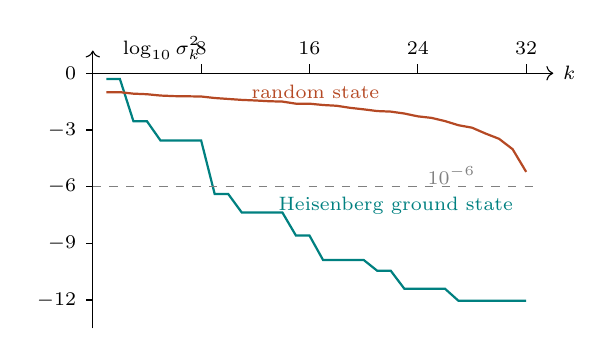
\begin{tikzpicture}[scale=1,x=0.215cm,y=0.30cm]
      \draw[->] (0,0) -- (34,0) node[right,dlab] {$k$};
      \draw[->] (0,-13.5) -- (0,1.2);
      \node[dlab,anchor=south west] at (1.5,0.2) {$\log_{10}\sigma_k^2$};
      \foreach \y in {0,-3,-6,-9,-12} \draw (0,\y) -- (-0.5,\y) node[left,dlab] {$\y$};
      \foreach \x in {8,16,24,32} \draw (\x,0) -- (\x,0.5) node[above,dlab] {$\x$};
      \draw[teal,thick] plot coordinates {(1,-0.30) (2,-0.30) (3,-2.54) (4,-2.54) (5,-3.56) (6,-3.56) (7,-3.56) (8,-3.56) (9,-6.39) (10,-6.39) (11,-7.37) (12,-7.37) (13,-7.37) (14,-7.37) (15,-8.59) (16,-8.59) (17,-9.88) (18,-9.88) (19,-9.88) (20,-9.88) (21,-10.45) (22,-10.45) (23,-11.40) (24,-11.40) (25,-11.40) (26,-11.40) (27,-12.04) (28,-12.04) (29,-12.04) (30,-12.04) (31,-12.04) (32,-12.04)};
      \draw[warm,thick] plot coordinates {(1,-1.00) (2,-1.00) (3,-1.08) (4,-1.11) (5,-1.18) (6,-1.21) (7,-1.22) (8,-1.23) (9,-1.31) (10,-1.36) (11,-1.41) (12,-1.44) (13,-1.48) (14,-1.50) (15,-1.61) (16,-1.61) (17,-1.68) (18,-1.72) (19,-1.83) (20,-1.91) (21,-2.00) (22,-2.03) (23,-2.13) (24,-2.28) (25,-2.36) (26,-2.53) (27,-2.75) (28,-2.88) (29,-3.19) (30,-3.47) (31,-4.02) (32,-5.22)};
      \node[dlab,warm,anchor=west] at (11,-1.0) {random state};
      \node[dlab,teal,anchor=west] at (13,-7.0) {Heisenberg ground state};
      \draw[dashed,gray] (0,-6) -- (33,-6);
      \node[dlab,gray,anchor=west] at (24,-5.4) {$10^{-6}$};
    \end{tikzpicture}
    \end{center}
    \centering\small\alert{Exponential decay is what makes the method work.}
  \end{columns}
\end{frame}

% ======================================================================
\section{Thursday, lecture 1 continued: The MPS, its bond dimension and its truncation}
% ======================================================================

\begin{frame}{Tensor-network diagrams (section 11.2)}
  A shape is a tensor, a leg is an index, a \emph{connected} leg is a summed index.
  \begin{center}
  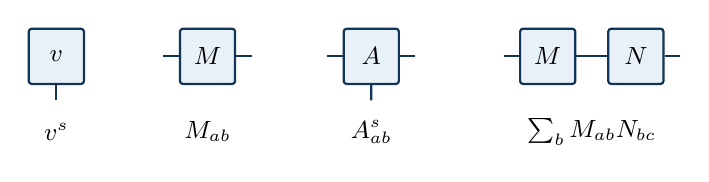
\begin{tikzpicture}[baseline]
    \node[tens] (v) at (0,0) {$v$}; \draw[leg] (v)--++(0,-0.7);
    \node at (0,-1.2) {\small $v^s$};
    \node[tens] (m) at (2.4,0) {$M$}; \draw[leg] (m)--++(-0.7,0); \draw[leg] (m)--++(0.7,0);
    \node at (2.4,-1.2) {\small $M_{ab}$};
    \node[tens] (a) at (5.0,0) {$A$}; \draw[leg] (a)--++(-0.7,0); \draw[leg] (a)--++(0.7,0); \draw[leg] (a)--++(0,-0.7);
    \node at (5.0,-1.2) {\small $A^{s}_{ab}$};
    \node[tens] (x) at (7.8,0) {$M$}; \node[tens] (y) at (9.2,0) {$N$};
    \draw[leg] (x)--++(-0.7,0); \draw[leg] (x)--(y); \draw[leg] (y)--++(0.7,0);
    \node at (8.5,-1.2) {\small $\sum_bM_{ab}N_{bc}$};
  \end{tikzpicture}
  \end{center}
  \begin{itemize}
    \item A closed diagram is a number; $k$ free legs is a $k$-index tensor
    \item Contracting two tensors costs the product of all their dimensions
    \item The \alert{order} of contractions decides the cost: $\chi^3$ or $\chi^4$
    \item Every SVD below is preceded by a \emph{reshape}
  \end{itemize}
\end{frame}

\begin{frame}{Building the MPS: SVD, $L-1$ times (section 11.2)}
  $\ket\Psi=\sum_{s_1\cdots s_L}C_{s_1\cdots s_L}\ket{s_1\cdots s_L}$: a tensor with $L$ legs, $d^L$ entries.
  \[
    C_{s_1,(s_2\cdots s_L)}
    =\sum_{a_1}\underbrace{U_{s_1a_1}}_{A^{s_1}_{a_1}}\sigma_{a_1}V^{\dagger}_{a_1,(s_2\cdots s_L)}
    \qquad\longrightarrow\qquad
    \text{reshape, SVD again, continue}
  \]
  \begin{block}{After $L-1$ steps}
    \[
      C_{s_1s_2\cdots s_L}=\Amat{s_1}\Amat{s_2}\cdots\Amat{s_L}
    \]
    $L$ matrices, one per site, \emph{selected} by the local index $s_i$; bond dimension 1 at the ends.
  \end{block}
  \begin{center}
  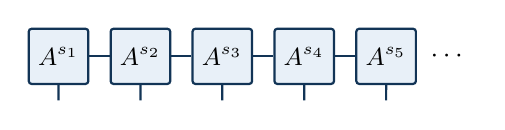
\begin{tikzpicture}[baseline]
    \foreach \i in {1,...,5}{\node[tens] (A\i) at (1.3*\i,0) {$A^{s_\i}$}; \draw[leg] (A\i)--++(0,-0.7);}
    \foreach \i [evaluate=\i as \j using int(\i+1)] in {1,...,4}{\draw[leg] (A\i)--(A\j);}
    \node at (1.3*5+1.0,0) {$\cdots$};
  \end{tikzpicture}
  \end{center}
  \centering\alert{Nothing has been approximated yet} -- the construction is exact for any state.
\end{frame}

\begin{frame}{What the bond index is (section 11.2)}
  \begin{columns}[T]
    \column{0.52\textwidth}
    $\Amat{s_i}$ has shape $\chi_{i-1}\times\chi_i$, with
    \[
      \chi_i=\min\bigl(d^{\,i},\ d^{\,L-i},\ \chi\bigr).
    \]
    \small
    \begin{itemize}
      \item The exact Schmidt rank of the cut at bond $i$
      \item Three arguments, three limits: left half, right half, our choice
      \item \alert{The profile is a tent}, peaking at $d^{L/2}$
      \item So $\chi_{i-1}\times\chi_i$ is right on \emph{both} halves
    \end{itemize}
    \column{0.44\textwidth}
    \begin{center}
    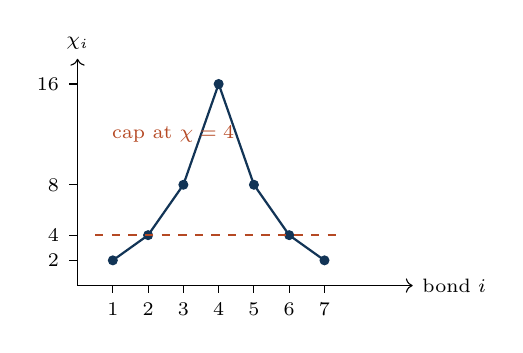
\begin{tikzpicture}[scale=1,x=0.56cm,y=0.40cm]
      \draw[->] (0,0) -- (9.5,0) node[right,dlab] {bond $i$};
      \draw[->] (0,0) -- (0,9) node[above,dlab] {$\chi_i$};
      \foreach \x/\l in {1/1,2/2,3/3,4/4,5/5,6/6,7/7} \draw (\x,0) -- (\x,-0.3) node[below,dlab] {\l};
      \foreach \y/\l in {1/2,2/4,4/8,8/16} \draw (0,\y) -- (-0.25,\y) node[left,dlab] {\l};
      \draw[uioblue,thick] plot coordinates {(1,1) (2,2) (3,4) (4,8) (5,4) (6,2) (7,1)};
      \filldraw[uioblue] (1,1) circle (2pt) (2,2) circle (2pt) (3,4) circle (2pt) (4,8) circle (2pt) (5,4) circle (2pt) (6,2) circle (2pt) (7,1) circle (2pt);
      \draw[warm,thick,dashed] (0.5,2) -- (7.5,2);
      \node[dlab,warm,anchor=west] at (0.7,6.0) {cap at $\chi=4$};
    \end{tikzpicture}
    \end{center}
    \centering\scriptsize $L=8$ qubits: $2,4,8,16,8,4,2$. A cap at $\chi=4$ touches only the three middle bonds.
  \end{columns}
\end{frame}

\begin{frame}{MPS by hand: GHZ and W (section 11.2; chapter 11, exercise 1)}
  \small
  \begin{block}{GHZ $(\ket{000}+\ket{111})/\sqrt2$ -- the bond index as a classical memory}
    \[
      \Amat0_1=\tfrac1{\sqrt2}(1,0),\quad \Amat1_1=\tfrac1{\sqrt2}(0,1),\quad
      \Amat0_2=\mathrm{diag}(1,0),\quad \Amat1_2=\mathrm{diag}(0,1),\quad
      \Amat0_3=\tbinom10,\quad \Amat1_3=\tbinom01
    \]
    Diagonal in the middle: the branch may not change. $\chi=2$, and no $\chi=1$ MPS can do it.
  \end{block}
  \begin{block}{W $(\ket{100}+\ket{010}+\ket{001})/\sqrt3$ -- the bond index as an automaton}
    \[
      \Amat0_2=\bmat I,\qquad \Amat1_2=\begin{pmatrix}0&1\\0&0\end{pmatrix}
      \qquad\Longrightarrow\qquad
      C_{110}=0
    \]
    State 1 = ``not placed yet'', state 2 = ``done''. \alert{Remember this} -- tomorrow it builds every operator.
  \end{block}
  \centering $\chi=1$ \emph{is} a product state; every bond dimension above one is entanglement.
\end{frame}

\begin{frame}{A physical state that is exactly an MPS: AKLT (section 11.2; chapter 11, exercise 3)}
  \small
  \[
    \hH=\sum_i\Bigl[\bm S_i\cdot\bm S_{i+1}+\tfrac13\bigl(\bm S_i\cdot\bm S_{i+1}\bigr)^2\Bigr]
  \]
  \[
    \bmat A^{+1}=\sqrt{\tfrac23}\begin{pmatrix}0&1\\0&0\end{pmatrix},\qquad
    \bmat A^{0}=-\sqrt{\tfrac13}\begin{pmatrix}1&0\\0&-1\end{pmatrix},\qquad
    \bmat A^{-1}=-\sqrt{\tfrac23}\begin{pmatrix}0&0\\1&0\end{pmatrix}
  \]
  Spin-1, $d=3$, $\chi=2$, and $\sum_s\bmat A^{s\dagger}\bmat A^s=\bmat I$: left-canonical as they stand.
  \begin{block}{Checked in a few lines of numpy (chapter 11, exercise 3d)}
    \begin{itemize}
      \item $\chi=2$ is \emph{exact} at every $L$: $\hH\ket\psi=E\ket\psi$ to $10^{-15}$, $E=-\tfrac23(L-1)$ on the open chain ($-\tfrac23L$ on a ring): $-\tfrac23$ per bond
      \item $S=\ln2$ on an open chain, $2\ln2$ on a ring -- \alert{the entropy counts boundaries}
      \item Transfer matrix eigenvalues $1$ and $-\tfrac13$: $\xi=1/\ln3=0.9102$
    \end{itemize}
  \end{block}
\end{frame}

\begin{frame}{Pause to think: bond dimension}
  \thinkq{4}{
  \begin{enumerate}
    \item GHZ and AKLT both have $\chi=2$ at any $L$, so both are cheap. Does that mean they are weakly entangled? What exactly is bounded?
    \item An MPS has $\approx Ld\chi^2$ parameters, the exact one needs $\chi=d^{L/2}$. For $L=12$, $d=4$: at what $\chi$ does the MPS stop being a saving?
  \end{enumerate}}
\end{frame}

\begin{frame}{Answer}
  \thinka{
  \begin{enumerate}
    \item Bounded is the entropy \emph{across a single cut}, $\ln2$ for both. GHZ superposes two macroscopic branches; AKLT has string order and spin-$\tfrac12$ edge modes. \alert{Cheap means few Schmidt states per cut, not ``nearly a product state''.}
    \item $\chi>\sqrt{4^{12}/48}=591$, while the exact MPS needs $4^6=4096$: an \emph{exact} MPS costs more than storing the tensor. The ansatz pays off only because real spectra decay.
  \end{enumerate}}
\end{frame}

\begin{frame}{Counting parameters, and truncation (section 11.2)}
  \[
    Ld\chi^2\ \text{parameters, \alert{linear in $L$}}
    \qquad\text{against}\qquad
    d^L .
  \]
  \begin{block}{The error you control}
    Keep the $\chi$ largest singular values at every bond: the best rank-$\chi$ approximation (Eckart--Young), with discarded weight
    \[
      \varepsilon_\chi=\sum_{k>\chi}\sigma_k^2 .
    \]
  \end{block}
  \begin{itemize}
    \item Report $\varepsilon_\chi$, not $\chi$
    \item \emph{Variational}: $E(\chi)\ge E_0$, improving monotonically with $\chi$
    \item \alert{The method computes its own error bar} -- an excitation level does not
  \end{itemize}
\end{frame}

\begin{frame}{Numerical check: truncating the exact state (section 11.2)}
  \begin{columns}[T]
    \column{0.46\textwidth}
    \begin{center}\small
    \begin{tabular}{@{}rlll@{}}\toprule
    $\chi$ & $\varepsilon_\chi$ & $E(\chi)$ & $E(\chi)-E_0$\\\midrule
    2 & $2.5\times10^{-1}$ & $-3.89820374$ & $3.6\times10^{-1}$\\
    4 & $2.7\times10^{-3}$ & $-4.25110973$ & $6.9\times10^{-3}$\\
    8 & $4.6\times10^{-6}$ & $-4.25801999$ & $1.5\times10^{-5}$\\
    16 & $6.2\times10^{-10}$ & $-4.25803520$ & $2.7\times10^{-9}$\\
    32 & 0 & $-4.25803521$ & 0\\\bottomrule
    \end{tabular}
    \end{center}
    \centering\scriptsize Heisenberg, $L=10$: exact MPS, then truncated bond by bond from the left; $\varepsilon_\chi$ summed over the nine bonds (section 11.2).
    \column{0.50\textwidth}
    \small
    \begin{itemize}
      \item The error is \emph{positive}: truncation can only raise the energy
      \item It is a few times $\varepsilon_\chi$ -- here $1.5$ to $4$. \alert{That is why $\varepsilon_\chi$ works as an error bar}
      \item Three to four decades per doubling of $\chi$
    \end{itemize}
  \end{columns}
\end{frame}

\begin{frame}{Where lecture 1 leaves us}
  \begin{block}{Established}
    \begin{itemize}
      \item A bipartite state is a matrix; its SVD is the Schmidt decomposition
      \item Area law: $S\sim\ell^{\mathcal D-1}$ -- constant in 1D, $\ln L$ if critical; generic states obey neither
      \item SVD at every bond $\Rightarrow$ MPS, exactly
      \item Truncation: best of its rank, variational, with a computable error
    \end{itemize}
  \end{block}
  \begin{block}{Missing}
    We built the MPS \emph{from} a state vector -- which we cannot have for large $L$.
    \begin{itemize}
      \item Tomorrow: working with an MPS without ever forming the vector
      \item Next week: \emph{finding} the ground state by sweeping (sections 11.5--11.6)
    \end{itemize}
  \end{block}
  \centering Exercises for this week: last frames -- the stability matrix by Wick's theorem, and positive semidefinite matrices.
\end{frame}

% ======================================================================
\section{Friday, lecture 2: Gauge freedom, canonical forms and contractions}
% ======================================================================

\begin{frame}{Gauge freedom (section 11.2)}
  \[
    \Amat{s_i}\to\Amat{s_i}\bmat X,\qquad \Amat{s_{i+1}}\to\bmat X^{-1}\Amat{s_{i+1}}
  \]
  leaves every coefficient unchanged: $\approx\chi^2$ redundant numbers per bond.
  \begin{center}
  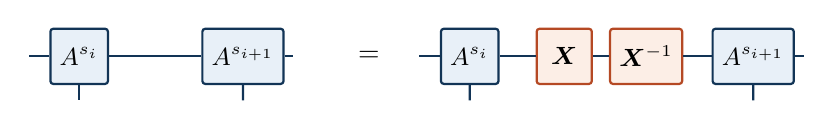
\begin{tikzpicture}[baseline]
    \node[tens] (A) at (0,0) {$A^{s_i}$}; \node[tens] (B) at (2.6,0) {$A^{s_{i+1}}$};
    \draw[leg] (A)--++(-0.8,0); \draw[leg] (A)--(B); \draw[leg] (B)--++(0.8,0);
    \draw[leg] (A)--++(0,-0.7); \draw[leg] (B)--++(0,-0.7);
    \node at (4.6,0) {$=$};
    \node[tens] (A2) at (6.2,0) {$A^{s_i}$}; \node[mpo] (X) at (7.7,0) {$\bmat X$};
    \node[mpo] (Xi) at (9.0,0) {$\bmat X^{-1}$}; \node[tens] (B2) at (10.7,0) {$A^{s_{i+1}}$};
    \draw[leg] (A2)--++(-0.8,0); \draw[leg] (A2)--(X); \draw[leg] (X)--(Xi); \draw[leg] (Xi)--(B2); \draw[leg] (B2)--++(0.8,0);
    \draw[leg] (A2)--++(0,-0.7); \draw[leg] (B2)--++(0,-0.7);
  \end{tikzpicture}
  \end{center}
  \begin{block}{Canonical forms}
    \[
      \text{left: }\sum_s\Amat{s\dagger}\Amat s=\bmat I,
      \qquad
      \text{right: }\sum_s\Bmat{s}\Bmat{s\dagger}=\bmat I,
    \]
    \[
      \text{mixed: }\quad C_{s_1\cdots s_L}=\Amat{s_1}\cdots\Amat{s_{i-1}}\,\bm\Theta^{s_is_{i+1}}\,\Bmat{s_{i+2}}\cdots\Bmat{s_L}
    \]
  \end{block}
  \centering\small Lecture 1 already produced a left-canonical MPS: it \emph{is} $\bmat U^{\dagger}\bmat U=\bmat I$, reshaped.
\end{frame}

\begin{frame}{Why canonical forms matter (section 11.2)}
  \[
    \ket{a_i}_L=\sum_{s_1\cdots s_i}\bigl(\Amat{s_1}\cdots\Amat{s_i}\bigr)_{a_i}\ket{s_1\cdots s_i}
    \qquad\Longrightarrow\qquad
    \braket{a_i}{a_i'}_L=\delta_{a_ia_i'}
  \]
  \centering\alert{The block states are orthonormal} -- $\chi_i$ of them instead of $d^{\,i}$.
  \begin{block}{In mixed-canonical form}
    \begin{itemize}
      \item Norm: $\braket\Psi\Psi=\|\bm\Theta\|_F^2$, no contraction of the chain
      \item The SVD of $\bm\Theta$ \emph{is} the Schmidt decomposition at that bond: entropy and truncation error \alert{for free}
      \item Local expectation values are traces against $\bm\Theta$
    \end{itemize}
  \end{block}
  \mbbox{In CI the block basis is determinants: orthonormal, but $\binom nN$ of them. Here each half has a basis \emph{adapted to the state} -- $\chi$ block states chosen by the SVD. That is the sense in which DMRG is a renormalisation group.}
\end{frame}

\begin{frame}{Pause to think: gauge and canonical forms}
  \thinkq{4}{
  \begin{enumerate}
    \item Gauge freedom removes $\approx\chi^2$ numbers per bond. How many parameters does the \emph{state} have?
    \item Left-canonical form can be reached by SVD or by QR. Why prefer QR?
    \item Show that a left-canonical MPS is automatically normalised.
  \end{enumerate}}
\end{frame}

\begin{frame}{Answer}
  \thinka{
  \begin{enumerate}
    \item $Ld\chi^2-(L-1)\chi^2\approx L\chi^2(d-1)$: the usual count overestimates by $d/(d-1)$. The redundancy buys trivial contractions.
    \item QR is cheaper and \emph{exact}: no singular values to inspect, nothing small to divide by. \alert{QR to move the gauge, SVD only where you truncate.}
    \item Contract from the left: $\sum_{s_1}\Amat{s_1\dagger}\Amat{s_1}=\bmat I$, absorb into the next pair, repeat. Canonicity does the normalisation -- which is why the AKLT tensors needed none.
  \end{enumerate}}
\end{frame}

\begin{frame}{Contractions: the cost is in the order (section 11.2)}
  \begin{center}
  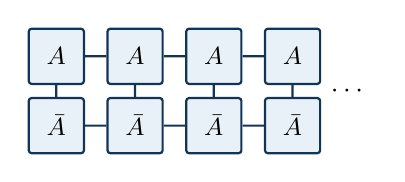
\begin{tikzpicture}[baseline]
    \foreach \i in {1,...,4}{
      \node[tens] (T\i) at (1.25*\i,0.55) {$A$};
      \node[tens] (B\i) at (1.25*\i,-0.55) {$\bar A$};
      \draw[leg] (T\i)--(B\i);}
    \foreach \i [evaluate=\i as \j using int(\i+1)] in {1,...,3}{\draw[leg] (T\i)--(T\j); \draw[leg] (B\i)--(B\j);}
    \node at (1.25*4+0.9,0) {$\cdots$};
  \end{tikzpicture}
  \end{center}
  Transfer matrix $\mathbb E=\sum_s\Amat s\otimes\overline{\Amat s}$, applied one site at a time.
  \begin{itemize}
    \item Column by column: $\bigO(L\chi^3d)$. An intermediate with three bond indices: $\chi^4$
    \item Never form the $d^L$ vector
    \item In mixed-canonical form a local $\hat O_i$ collapses to $\bm\Theta,\hat O_i,\bar{\bm\Theta}$: the rest cancels
    \item So $\langle\hat n_p\rangle$ and $\langle\bm S_i\cdot\bm S_{i+1}\rangle$ are free once the sweep passes
  \end{itemize}
  \centering\alert{The most important practical habit in tensor-network computing.}
\end{frame}

\begin{frame}{Numerical check: the AKLT transfer matrix (section 11.2)}
  \begin{columns}[T]
    \column{0.46\textwidth}
    $\mathbb E=\sum_s\bmat A^s\otimes\bmat A^s$ is $4\times4$, eigenvalues $\{1,-\tfrac13,-\tfrac13,-\tfrac13\}$.
    \vspace{0.4em}
    \small
    \begin{itemize}
      \item $\lambda_1=1$ \emph{must} hold: canonicity as an eigenvalue equation
      \item $\xi=-1/\ln|\lambda_2|=1/\ln3$
      \item $\lambda_2<0$: alternating sign
    \end{itemize}
    \column{0.50\textwidth}
    \begin{center}\small
    \begin{tabular}{@{}rrr@{}}\toprule
    $r$ & $\langle S^z_2S^z_{2+r}\rangle$ & $\frac43(-\frac13)^r$\\\midrule
    1 & $-0.444505$ & $-0.444444$\\
    2 & $+0.148349$ & $+0.148148$\\
    3 & $-0.049992$ & $-0.049383$\\
    4 & $+0.018290$ & $+0.016461$\\\bottomrule
    \end{tabular}
    \end{center}
    \centering\scriptsize Open chain, $L=10$: the deviation grows as the pair approaches the end.
  \end{columns}
  \vspace{0.6em}
  \centering A finite $\chi$ \emph{forces} exponential decay -- so a critical chain is never an exact MPS.
\end{frame}

% ======================================================================
\section{Friday, lecture 2 continued: Matrix product operators and fermions}
% ======================================================================

\begin{frame}{Matrix product operators (section 11.3)}
  \[
    \hH=\sum_{\{s\},\{s'\}}\bmat W^{s_1s_1'}\bmat W^{s_2s_2'}\cdots\bmat W^{s_Ls_L'}\;\ket{s_1\cdots s_L}\bra{s_1'\cdots s_L'}
  \]
  $\bmat W_i$ is $D_{i-1}\times D_i$, and each \emph{entry} is a $d\times d$ operator.
  \begin{center}
  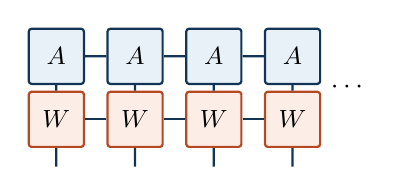
\begin{tikzpicture}[baseline]
    \foreach \i in {1,...,4}{
      \node[tens] (A\i) at (1.25*\i,1.0) {$A$};
      \node[mpo] (W\i) at (1.25*\i,0.0) {$W$};
      \draw[leg] (A\i)--(W\i); \draw[leg] (W\i)--++(0,-0.75);}
    \foreach \i [evaluate=\i as \j using int(\i+1)] in {1,...,3}{\draw[leg] (A\i)--(A\j); \draw[leg] (W\i)--(W\j);}
    \node at (1.25*4+0.9,0.5) {$\cdots$};
  \end{tikzpicture}
  \end{center}
  \begin{itemize}
    \item $\hH\ket\Psi$ is again an MPS, with bond dimension $\chi D$
    \item \emph{Automaton:} a machine walks the chain, placing operators, remembering what is open
    \item \alert{$D$ counts the partial terms open at a cut} -- not the terms in $\hH$
  \end{itemize}
\end{frame}

\begin{frame}{The Heisenberg chain: $D=5$ (section 11.3)}
  \[
    \hH=J\sum_i\bm S_i\cdot\bm S_{i+1},
    \qquad
    \bmat W=\begin{pmatrix}
      \hat1 & S^x & S^y & S^z & 0\\
      0&0&0&0&JS^x\\
      0&0&0&0&JS^y\\
      0&0&0&0&JS^z\\
      0&0&0&0&\hat1
    \end{pmatrix}
  \]
  \centering First site: the first row. Last site: the last column.
  \begin{itemize}
    \item The five states: nothing placed; $S^x$, $S^y$ or $S^z$ waiting for a partner; finished
    \item Each path $1\to\alpha\to5$ places exactly one bond term
    \item Ising: $D=3$. AKLT: $D=14$, since the biquadratic term must remember which of \emph{nine} pairs $(\alpha,\beta)$ is open, $1+3+9+1$
  \end{itemize}
\end{frame}

\begin{frame}{The pairing model: $D=4$, though every level couples to every other (section 11.3)}
  \[
    \hH=\sum_p\varepsilon_p\hat n_p-\frac g2\sum_{pq}\hat P^+_p\hat P^-_q,
    \qquad
    \bmat W_p=\begin{pmatrix}
      \hat1 & \hat P^+_p & \hat P^-_p & \varepsilon_p\hat n_p-\frac g2\hat n_{p+}\hat n_{p-}\\
      0&\hat1&0&-\frac g2\hat P^-_p\\
      0&0&\hat1&-\frac g2\hat P^+_p\\
      0&0&0&\hat1
    \end{pmatrix}
  \]
  \begin{itemize}
    \item $1\to4$: one-body and $p=q$; \quad $1\to2\to4$: $q>p$; \quad $1\to3\to4$: $q<p$
    \item The $\hat1$ on the diagonal \emph{carries} an open term across any distance
    \item \alert{Long range is free here}: the interaction factorises, $v_{pq}$ has rank one
    \item A general two-body interaction does not -- then $D$ grows and ordering matters
  \end{itemize}
\end{frame}

\begin{frame}{Three more, and the systematic route (section 11.3)}
  \begin{columns}[T]
    \column{0.46\textwidth}
    \begin{block}{Bond dimensions to know}
      \begin{itemize}
        \item Hubbard chain: $D=6$ (ring: $10$)
        \item Penalty $\lambda(\hat N-N_0)^2$: $D=3$
        \item Particle--hole term: $D=14$
        \item Range-$r$ hopping: $D=2r+2$
      \end{itemize}
    \end{block}
    \column{0.50\textwidth}
    \begin{block}{Do not write automata by hand for long}
      Write $\hH=\sum_kc_k\,\hat o^{(k)}_1\cdots\hat o^{(k)}_L$, form at each cut the matrix of left parts against right parts, and compress it with an SVD: its rank \emph{is} the minimal $D$.
    \end{block}
  \end{columns}
  \vspace{0.5em}
  \warnbox{Build the MPO and the exact-diagonalisation reference from the \emph{same} operator-string list. Then the two solvers cannot disagree about a sign, and any discrepancy is a real bug.}
\end{frame}

\begin{frame}{Adding, applying, compressing (section 11.4)}
  \small
  \begin{columns}[T]
    \column{0.5\textwidth}
    \begin{block}{Two exact operations that grow $\chi$}
      \begin{itemize}
        \item Sum: $\bmat N^{s}=\bmat M^{s}\oplus\tilde{\bmat M}^{s}$ (block diagonal), bond dimensions \emph{add}
        \item MPO on MPS: $N^{s}_{(ba),(b'a')}=\sum_{s'}W^{ss'}_{bb'}M^{s'}_{aa'}$, bond dimension $D\chi$, cost $\bigO(Ld^2D^2\chi^2)$
        \item $\hat H^2$: an MPO of dimension $\le D^2$, compressible ($9$, not $25$, for Heisenberg)
      \end{itemize}
    \end{block}
    \column{0.48\textwidth}
    \begin{block}{One approximate operation that shrinks it}
      \begin{itemize}
        \item SVD compression: sweep, truncate every bond; fast, one-sided errors
        \item Variational: minimise $\|\ket\psi-\ket{\tilde\psi}\|^2$ one tensor at a time; in mixed-canonical form the update is explicit, $\tilde{\bmat M}=\mathcal L\,\bmat M\,\mathcal R$, no linear system
        \item Seed the second with the first; two-site updates avoid getting stuck
      \end{itemize}
    \end{block}
  \end{columns}
  \vspace{0.4em}
  \centering MPS of fixed $\chi$ are not closed under $+$ or under $\hat H$; \alert{compression is where every MPS algorithm makes its approximation.}
\end{frame}

\begin{frame}{Pause to think: what the bond dimension counts}
  \thinkq{4}{
  \begin{enumerate}
    \item An $L=100$ Heisenberg chain has $297$ terms, and $D=5$. Explain the discrepancy in one sentence.
    \item What is $D$ for $J_1\sum_i\bm S_i\cdot\bm S_{i+1}+J_2\sum_i\bm S_i\cdot\bm S_{i+2}$?
    \item Pairing couples every level to every other and still has $D=4$. What property does the work? Would a general $\sum_{pqrs}\element{pq}{\hat v}{rs}\ad p\ad qa_sa_r$ keep it?
  \end{enumerate}}
\end{frame}

\begin{frame}{Answer}
  \thinka{
  \begin{enumerate}
    \item $D$ counts terms open \emph{at one cut}, and at most one bond term straddles a cut; the $297$ terms are \emph{paths} through the network, not its width.
    \item $D=8$: each component now needs two waiting states, $1+3+3+1$.
    \item \alert{Factorisation:} $\sum_{pq}\hat P^+_p\hat P^-_q=(\sum_p\hat P^+_p)(\sum_q\hat P^-_q)$, i.e.\ $v_{pq}$ has rank one. A general interaction needs one open index per straddling pair, so $D=\bigO(L^2)$ for chemistry. Pairing is lucky, and we can name the reason.
  \end{enumerate}}
\end{frame}

\begin{frame}{Fermions on a chain: Jordan--Wigner (section 11.7; chapter 3, section 3.18)}
  An MPS describes \emph{distinguishable} sites, so antisymmetry is put in by hand:
  \[
    \ad m\ \longrightarrow\ (\text{local raising operator})\times\prod_{m'<m}(-1)^{\hat n_{m'}} .
  \]
  In practice: one site per level, $d=4$, carrying $\hat F=(-1)^{\hat n_++\hat n_-}$ on every site to the left.
  \begin{itemize}
    \item Pairing: the strings \alert{cancel} -- $\hat P^{\pm}_p$ has both operators on the same site
    \item Hubbard and particle--hole: strings are real, but cost \emph{no} bond dimension
    \item What they cost is \alert{locality}: on a ring or in 2D, a local interaction becomes a string of length $\bigO(L)$
  \end{itemize}
  \centering That is a large part of why the DMRG is a one-dimensional method.
\end{frame}

\begin{frame}{Summary of week 40}
  \small
  \begin{columns}[T]
    \column{0.48\textwidth}
    \begin{block}{Thursday: the ansatz}
      \begin{itemize}
        \item A state is a matrix; its SVD is the Schmidt decomposition; $\bmat U,\bmat V$ are isometries
        \item Area law: $S\sim\ell^{\mathcal D-1}$; constant only in $\mathcal D=1$, $\ln L$ if critical
        \item SVD at every bond $\Rightarrow$ MPS, $\chi_i=\min(d^i,d^{L-i},\chi)$
        \item $Ld\chi^2$ parameters; $\varepsilon_\chi$ is the error bar
      \end{itemize}
    \end{block}
    \column{0.48\textwidth}
    \begin{block}{Friday: the technology}
      \begin{itemize}
        \item Canonical forms fix the gauge: orthonormal block states
        \item Mixed-canonical: norm $=\|\bm\Theta\|_F^2$, entropies free
        \item Contract in the right order: $\bigO(L\chi^3d)$
        \item MPO $=$ automaton; $D$ counts open terms: $5,4,3,6,14,2r+2$
        \item Jordan--Wigner: free in $D$, expensive in locality
      \end{itemize}
    \end{block}
  \end{columns}
\end{frame}

% ======================================================================
\section{Exercises: week 40, and answers for week 39}
% ======================================================================

\begin{frame}{Exercise session: week 40 (suggested set)}
  \footnotesize
  Two exercises on the stability matrix of week 39, done with Wick's theorem and with linear algebra. Both are new and are answered on next week's slides.
  \begin{block}{Exercise 1: the stability matrix from Wick's theorem (section 6.10; new)}
    Write $\hat H=E_0+\hat F_N+\hat V_N$, normal ordered with respect to the Hartree-Fock determinant $\ket{c}$, with $f_{pq}=\varepsilon_p\delta_{pq}$ in the Hartree-Fock basis.
    \begin{enumerate}
      \item[a)] Show $\braket{c'}{c'}=1+\sum_{ai}|\delta C_{ai}|^2+\bigO(\delta C^3)$ for $\ket{c'}=e^{\hat T}\ket{c}$, saying which terms of $e^{\hat T}=\prod_i(1+\hat T_i)$ are second order.
      \item[b)] Evaluate $\element{c}{\nc{a_i^{\dagger}a_a}\,\hat F_N\,\nc{a_b^{\dagger}a_j}}{c}$ with Wick's theorem: draw the two complete contraction patterns, fix their signs, and show that the result is $f_{ab}\delta_{ij}-f_{ji}\delta_{ab}=(\varepsilon_a-\varepsilon_i)\delta_{ab}\delta_{ij}=\Delta_{ai,bj}$.
      \item[c)] Evaluate $\element{c}{\nc{a_i^{\dagger}a_a}\,\hat V_N\,\nc{a_b^{\dagger}a_j}}{c}$: four complete contraction patterns, all equal by the antisymmetry of $\element{pq}{\hat v}{rs}$, and the result is $A_{ai,bj}=\element{aj}{\hat v}{ib}_{\mathrm{AS}}=-\element{aj}{\hat v}{bi}_{\mathrm{AS}}$. Do the sign of one pattern in full.
      \item[d)] Evaluate $\element{c}{\hat V_N\,a_a^{\dagger}a_i\,a_b^{\dagger}a_j}{c}$ and show that it equals $\element{ij}{\hat v}{ab}_{\mathrm{AS}}=B^{*}_{ai,bj}$, that $E_0$ and $\hat F_N$ contribute nothing to it, and that it vanishes unless $a\ne b$ and $i\ne j$.
      \item[e)] Assemble $\Delta E=\frac12\bra{\chi}\hat M\ket{\chi}$, verify that $\hat M$ is Hermitian, and check that for a single pair $(a,i)$ it reduces to the curvature $\element{\Phi_i^a}{\hat H}{\Phi_i^a}-E_0=\varepsilon_a-\varepsilon_i-\element{ai}{\hat v}{ai}$ of week 39, Thursday, with $B_{ai,ai}=\element{aa}{\hat v}{ii}=0$.
    \end{enumerate}
  \end{block}
\end{frame}

\begin{frame}{Exercise 2: the stability condition and positive semidefinite matrices (new)}
  \scriptsize
  \begin{block}{Reminder}
    A Hermitian matrix $\hat M$ is \emph{positive semidefinite}, $\hat M\ge0$, if $\bra{\chi}\hat M\ket{\chi}\ge0$ for every $\chi$. Equivalent statements: every eigenvalue is $\ge0$; $\hat M=\bm C^{\dagger}\bm C$ for some $\bm C$; \emph{every} principal minor (the determinant of every principal submatrix, not only the leading ones) is $\ge0$. \alert{Necessary but not sufficient} conditions, each a consequence of the definition and cheap to check: every diagonal element $M_{kk}\ge0$; every $2\times2$ principal minor $M_{kk}M_{ll}-|M_{kl}|^2\ge0$; $\tr\hat M\ge0$; $\det\hat M\ge0$; every principal submatrix is itself $\ge0$. Sylvester's criterion -- all \emph{leading} principal minors $>0$ -- characterises positive \emph{definite} matrices; with $\ge0$ it is only necessary.
  \end{block}
  \begin{enumerate}
    \item[a)] Show that $\bra{\chi}\hat M\ket{\chi}\ge0$ for all $\chi$ is equivalent to all eigenvalues being non-negative, and that $\hat M=\bm C^{\dagger}\bm C$ implies it. Which of the two is the statement ``$\Delta E\ge0$ in every direction of the manifold of determinants''?
    \item[b)] Show that $\mathrm{diag}(0,-1)$ has all leading principal minors $\ge0$ and is not positive semidefinite. Explain why $\Delta+A\ge0$, the necessary condition of week 39, is the ``principal submatrix'' condition, and why the diagonal condition $\varepsilon_a-\varepsilon_i+A_{ai,ai}\ge0$ is weaker still.
    \item[c)] Lipkin model with $N=2$, $\varepsilon$, $V$, $W=0$: the two $1p$-$1h$ pairs give a $4\times4$ matrix $\hat M$ with $\Delta+A=\varepsilon\bm 1$ and $B=\begin{psmallmatrix}0&V\\V&0\end{psmallmatrix}$. Write $\hat M$ out, check the conditions of the reminder one by one, and find the first one that fails as $|V|$ grows. Compare with the eigenvalues $\varepsilon\pm V$ and with $\chi=|V|(N-1)/\varepsilon$.
    \item[d)] Pairing model: a $2\times2$ block of $\hat M$ is $\begin{psmallmatrix}\Delta&-g/2\\-g/2&\Delta\end{psmallmatrix}$ with $\Delta=\varepsilon_q-\varepsilon_p+g/2$. Check the $2\times2$ minor and find the eigenvalues. Why does the interaction cancel exactly in the lower one, and what does that say about breaking a pair coherently?
    \item[e)] Suppose $\Delta+A$ itself has a negative eigenvalue. What does the corresponding eigenvector mean physically, what would a CIS calculation on this reference return, and why is this case ``worse'' than an instability that appears only through $B$?
  \end{enumerate}
\end{frame}

\begin{frame}{Answers to the week-39 exercises: 1, varying one orbital}
  \footnotesize
  \begin{block}{1a) Only components towards unoccupied orbitals matter}
    Insert $\phi_i+\sum_\lambda d_\lambda\phi_\lambda$ in row $i$ and use linearity in that row: the component $d_j\phi_j$ with $j\le F$, $j\ne i$, produces a determinant with two identical rows, which vanishes; $d_i\phi_i$ rescales $\Phi_0$ by $1+d_i$. What is left is $\Phi_0+\sum_{a>F}d_a\Phi_i^a$, and since the $\Phi_i^a$ are orthonormal and orthogonal to $\Phi_0$, $N_i^{-2}=1+\sum_a|d_a|^2$.
  \end{block}
  \begin{block}{1b) The expansion, and what a real $\eta$ misses}
    $E(\eta)=\bigl[E_0+\eta^{*}f_{ai}+\eta f_{ia}+|\eta|^2H_{aa}\bigr]/(1+|\eta|^2)$ with $H_{aa}=\element{\Phi_i^a}{\hat H}{\Phi_i^a}$. With $(1+|\eta|^2)^{-1}=1-|\eta|^2+\bigO(|\eta|^4)$,
    \[
      E(\eta)=E_0+2\,\mathrm{Re}(\eta f_{ia})+|\eta|^2(H_{aa}-E_0)-2|\eta|^2\,\mathrm{Re}(\eta f_{ia})+\bigO(|\eta|^4),
    \]
    the cubic term being the product of the linear term and $-|\eta|^2$. Stationarity needs $\mathrm{Re}(\eta f_{ia})=0$ for all $\eta$; a real $\eta$ fixes $\mathrm{Re}f_{ia}=0$ and leaves $\mathrm{Im}f_{ia}$ free.
  \end{block}
\end{frame}

\begin{frame}{Answers to the week-39 exercises: 1, continued}
  \footnotesize
  \begin{block}{1c) $\element{\Phi_0}{\hat V_N}{\Phi_i^a}=0$ without Wick, and the block-diagonal Fock matrix}
    Write $\hat V_N$ in the particle-hole form of week 37: each term is a normal-ordered product of $k$ quasi-particle creators and $4-k$ quasi-particle annihilators (a hole annihilator $a_i^{\dagger}$ counts as a creator, and so on). $\bra{\Phi_0}$ is the quasi-particle vacuum, so any creator standing to the left kills the matrix element; only the term with four annihilators survives, and it needs four quasi-particles to annihilate. $\ket{\Phi_i^a}$ has two. Hence zero. -- With $f_{ai}=0$ for all pairs the Fock matrix in the basis (occupied first) is block diagonal, $\bm f=\mathrm{diag}(\bm f_{\mathrm{oo}},\bm f_{\mathrm{uu}})$; diagonalising $\bm f_{\mathrm{oo}}$ mixes occupied orbitals among themselves, which changes $\ket{\Phi_0}$ by a phase (section 6.3), and diagonalising $\bm f_{\mathrm{uu}}$ does not touch it. Neither step disturbs $f_{ai}=0$.
  \end{block}
  \begin{block}{1d) The plot}
    For the random Hamiltonian the picture is the one of week 39's numerical-check frame: in the original basis $E(\eta)-E_0$ is a straight line of slope $2f_{ia}$ through the origin, bent by the quadratic term; its odd part equals $2\eta f_{ia}$ to within the cubic term $-2\eta^3f_{ia}$; a purely imaginary $\eta$ gives no linear change because $f_{ia}$ is real. In the Hartree-Fock basis the slope is zero to the SCF tolerance and $E(\eta)-E_0=\eta^2(H_{aa}-E_0)+\bigO(\eta^4)$, a parabola whose curvature is the diagonal element of the stability matrix for that pair. (Trap system, for comparison: slope $-0.867$ at $(a,i)=(4,2)$ in the oscillator basis, $-1.7\times10^{-10}$ in the Hartree-Fock basis.)
  \end{block}
\end{frame}

\begin{frame}{Answers to the week-39 exercises: 2, single-particle energies and Thouless}
  \footnotesize
  \begin{block}{2a) $E^{\mathrm{HF}}\ne\sum_i\varepsilon_i$}
    Multiply the Hartree-Fock equation $\sum_\beta h^{\mathrm{HF}}_{\alpha\beta}C_{i\beta}=\varepsilon_iC_{i\alpha}$ by $C_{i\alpha}^{*}$, sum over $\alpha$ and $i\le F$: $\sum_i\varepsilon_i=\sum_i\element{i}{\hat h_0}{i}+\sum_{ij}\element{ij}{\hat v}{ij}_{\mathrm{AS}}$. The energy functional carries $\frac12$ on the interaction, so $E^{\mathrm{HF}}=\sum_i\varepsilon_i-\frac12\sum_{ij}\element{ij}{\hat v}{ij}_{\mathrm{AS}}$: the interaction is counted once per partner in the sum of eigenvalues. In the notebook, $\sum_i\varepsilon_i-\frac12\sum_{ij}\element{ij}{\hat v}{ij}$ agrees with $E^{\mathrm{HF}}$ to $10^{-12}$ for the trap system.
  \end{block}
  \begin{block}{2b) Koopmans}
    Removing orbital $k$ with the others frozen: $E(N)-E(N-1)=\element{k}{\hat h_0}{k}+\sum_{j\ne k}\element{kj}{\hat v}{kj}_{\mathrm{AS}}=\varepsilon_k$ (the $j=k$ term vanishes by antisymmetry). Adding a particle in $a$ gives $E(N+1)-E(N)=\varepsilon_a$ by the same algebra, but $\varepsilon_a$ was computed in the field of \emph{all $N$} particles, whereas the added particle should feel the other $N$ and the occupied orbitals should relax around it; virtual orbitals are optimised for nothing, and the relaxation error is larger than for removal, where the orbital was at least self-consistent.
  \end{block}
\end{frame}

\begin{frame}{Answers to the week-39 exercises: 2, continued}
  \footnotesize
  \begin{block}{2c) $[a_a^{\dagger}a_i,a_b^{\dagger}a_j]=0$, $\hat T_i^2=0$, and the cross terms}
    With $i\ne b$: $a_ia_b^{\dagger}=-a_b^{\dagger}a_i$, so $a_a^{\dagger}a_ia_b^{\dagger}a_j=-a_a^{\dagger}a_b^{\dagger}a_ia_j$. With $j\ne a$: $a_b^{\dagger}a_ja_a^{\dagger}a_i=-a_b^{\dagger}a_a^{\dagger}a_ja_i=-a_a^{\dagger}a_b^{\dagger}a_ia_j$, the last step swapping both pairs (two signs). Equal, so the commutator vanishes; disjointness of the index sets is what prevented a $\delta$ from appearing in either anticommutation. $\hat T_i^2=\sum_{ab}C_{ai}C_{bi}a_a^{\dagger}a_ia_b^{\dagger}a_i=-\sum_{ab}C_{ai}C_{bi}a_a^{\dagger}a_b^{\dagger}a_ia_i=0$, hence $e^{\hat T_i}=1+\hat T_i$ and $e^{\hat T}=\prod_i(1+\hat T_i)$. The cross term $\hat T_i\hat T_j=\sum_{ab}C_{ai}C_{bj}a_a^{\dagger}a_b^{\dagger}a_ja_i$ ($i\ne j$) is a $2p$-$2h$ excitation with amplitude $C_{ai}C_{bj}-C_{bi}C_{aj}$ after antisymmetrisation: products of singles, no freedom of their own.
  \end{block}
  \begin{block}{2d) $\braket{c}{\tilde c}=\det(f_{ip})$}
    $N=2$: $\bra0a_2a_1\bigl(\sum_pf_{1p}a_p^{\dagger}\bigr)\bigl(\sum_qf_{2q}a_q^{\dagger}\bigr)\ket0$; only $p,q\in\{1,2\}$ survive and $\bra0a_2a_1a_p^{\dagger}a_q^{\dagger}\ket0=\delta_{p1}\delta_{q2}-\delta_{p2}\delta_{q1}$, giving $f_{11}f_{22}-f_{12}f_{21}$. In general every $a_p^{\dagger}$ must carry an occupied index and be contracted with a distinct $a_{i_k}$; summing over assignments with their signs is $\sum_\pi\sgn(\pi)\prod_kf_{i_k\pi(i_k)}=\det(f)$ over the occupied block. The proof inverts that block, so $\det\ne0$ is exactly what it needs; if it vanishes, $\ket{\tilde c}$ is orthogonal to $\ket c$ and not in its neighbourhood at all.
  \end{block}
\end{frame}

\begin{frame}{Answers to the week-39 exercises: 3, stability}
  \footnotesize
  \begin{block}{3a) The norm}
    $\ket{c'}=\{1+\sum\delta C_{ai}a_a^{\dagger}a_i+\frac12\sum\delta C_{ai}\delta C_{bj}a_a^{\dagger}a_ia_b^{\dagger}a_j+\cdots\}\ket c$. Zeroth order: $1$. Constant times linear: $\element{c}{a_a^{\dagger}a_i}{c}=0$. Linear times linear: $\sum\delta C^{*}_{ai}\delta C_{bj}\braket{\Phi_i^a}{\Phi_j^b}=\sum|\delta C_{ai}|^2$. Constant times quadratic: $\element{c}{a_a^{\dagger}a_ia_b^{\dagger}a_j}{c}=0$. Linear times quadratic is third order, quadratic times quadratic fourth. Hence $1+\sum|\delta C|^2+\bigO(\delta C^3)$.
  \end{block}
  \begin{block}{3b) $\Delta E$, the doubled vector, Hermiticity, the necessary condition}
    Subtract $(1+\sum|\delta C|^2)E_0$ from the second-order energy and divide by the norm: what remains over the norm is $\Delta E$. The $\delta C^{*}\delta C$ terms are $\delta C^{\dagger}(\Delta+A)\delta C$, the $\delta C^{*}\delta C^{*}$ terms $\frac12\delta C^{\dagger}B\,\delta C^{*}$, the $\delta C\,\delta C$ terms $\frac12\delta C^{T}B^{*}\delta C$; stacking $\chi=(\delta C,\delta C^{*})$ writes all three as $\frac12\bra\chi\hat M\ket\chi$. Hermitian: $(\Delta+A)_{bj,ai}=\element{bi}{\hat v}{ja}=\element{aj}{\hat v}{ib}^{*}=(\Delta+A)^{*}_{ai,bj}$ and $B_{bj,ai}=\element{ba}{\hat v}{ji}=B_{ai,bj}$, so the lower-left block is $B^{*}=B^{\dagger}$ and $\hat M^{\dagger}=\hat M$. Restricting $\chi$ to $(\delta C,0)$ -- allowed, since $\bra\chi\hat M\ket\chi\ge0$ must hold for every $\chi$ -- gives $\delta C^{\dagger}(\Delta+A)\delta C\ge0$: necessary; not sufficient, because a general $\chi$ also feels $B$.
  \end{block}
\end{frame}

\begin{frame}{Answers to the week-39 exercises: 3, continued}
  \footnotesize
  \begin{block}{3c) Lipkin, $W=0$}
    $\frac V2(\hat J_+^2+\hat J_-^2)$ changes $J_z$ by $\pm2$, so it has no element inside the $1p$-$1h$ space: $A=0$, $\Delta=\varepsilon\bm1$. $\hat J_-^2$ connects the reference to the $2p$-$2h$ state with pairs $p$ and $q$ both raised, so $B_{p,q}=V$ for $p\ne q$ and $0$ for $p=q$: $\bm B=V(\bm J-\bm 1)$, eigenvalues $V(N-1)$ once and $-V$ $(N-1)$ times. With $\hat M=\begin{psmallmatrix}\varepsilon\bm1&\bm B\\\bm B&\varepsilon\bm1\end{psmallmatrix}$ the eigenvalues are $\varepsilon\pm b$, and the smallest is $\varepsilon-|V|(N-1)=\varepsilon(1-\chi)$.
  \end{block}
  \begin{block}{3d) Pairing, four levels, four particles: $\lambda_{\min}(\hat M)=1$ for every $g$}
    The pairing interaction moves pairs, never a single particle: $A=0$. Breaking the pair at $p$ to put one particle in $q$ costs $\varepsilon_q-\varepsilon_p$ plus the lost pairing energy $g/2$: $\Delta=\varepsilon_q-\varepsilon_p+g/2$, and $\lambda_{\min}(\Delta+A)=1+g/2>0$. $B$ connects $\delta C_{q\uparrow,p\uparrow}$ with $\delta C^{*}_{q\downarrow,p\downarrow}$ through $\element{q\!\uparrow q\!\downarrow}{\hat v}{p\!\uparrow p\!\downarrow}=-g/2$, so $\hat M$ splits into $2\times2$ blocks $\begin{psmallmatrix}\Delta&-g/2\\-g/2&\Delta\end{psmallmatrix}$ with eigenvalues $\Delta\mp g/2=\varepsilon_q-\varepsilon_p$ and $\varepsilon_q-\varepsilon_p+g$. Moving the two members of a pair \emph{together} costs exactly the level spacing; the interaction cancels; the minimum is $\varepsilon_3-\varepsilon_2=1$ for all $g$ (notebook: $1.0000$ from $g=0.25$ to $3$). Stable, and useless: no number-conserving mean field captures pairing, which is why chapter 7 breaks particle number (BCS) and why the DMRG of this week, which keeps it, has to carry the correlation in its bond dimension instead.
  \end{block}
\end{frame}

\begin{frame}{Next week, and a closing remark}
  \begin{exampleblock}{Week 41: lectures 3 and 4}
    \small
    \textbf{Thursday:} the variational principle on the MPS manifold; environments and the effective Hamiltonian; the two-site update, Lanczos and SVD; extrapolation in $\varepsilon_\chi$.\\
    \textbf{Friday:} the pairing model, where the DMRG \emph{discovers} seniority zero; the Hubbard chain past exact diagonalisation; TEBD, where Trotter--Suzuki returns; the limits in 2D and in chemistry.\\
    Reading: chapter 11, sections 11.5--11.6 (the sweep, and White's original blocks and superblocks), 11.8--11.12; Schollw\"ock, Annals of Physics 326, 96 (2011), sections 2 and 6.
  \end{exampleblock}
  \vspace{0.6em}
  One idea did all the work: the singular value decomposition. Applied once it is the Schmidt decomposition; applied at every bond it turns $d^L$ amplitudes into $L$ small matrices, with the optimal truncation and a computable error.
  \vspace{0.6em}

  \centering\alert{Next week we stop \emph{building} matrix product states, and start \emph{finding} them.}
\end{frame}

\end{document}
